\deftripstyle{Flughandbuch}[.5pt][.5pt]{\pagemark}{}{\headmark}{Flug- und Betriebshandbuch B13}{}{LBA-anerkannt 06.2022}
\pagestyle{Flughandbuch}
\renewcommand*\chapterpagestyle{Flughandbuch}


\chapter{ Betriebsgrenzen}

\section{Einführung}
Der vorliegende Abschnitt beinhaltet Betriebsgrenzen, Instrumentenmarkierungen und Hinweisschilder, die für den sicheren Betrieb der B13 notwendig sind. 

\section{Fluggeschwindigkeiten}

Die Fluggeschwindigkeitsgrenzen und ihre Bedeutung für den Betrieb sind nachfolgend aufgeführt:

\begin{longtable}{|p{0.11\textwidth}|m{0.25\textwidth}|p{0.15\textwidth}|m{0.35\textwidth}|llll}
\hline
& Geschwindigkeit & IAS [$\unit{\frac{km}{h}}$] & Anmerkungen \\
\hline
$V_{NE}$ & Zulässige Höchst"-ge"-schwin"-digkeit bei ruhigem Wetter & $220$ & Diese Geschwindigkeit darf nicht überschritten werden und der Ruderausschlag darf nicht mehr als $\frac{1}{3}$ betragen\\
\hline
$V_{RA}$ & Zulässige Höchstge"-schwindigkeit in starker Turbulenz & $180$ & Diese Geschwindigkeit darf bei starker Turbulenz nicht überschritten werden. (Starke Turbulenz herrscht vor in Leewellen-Rotoren, Gewitterwolken, usw.) \\
\hline
$V_A$ & Manöver"-geschwindigkeit & $180$ & Oberhalb dieser Geschwindigkeit dürfen keine vollen oder abrupten Ruderausschläge ausgeführt werden, da die Flugzeugstruktur dabei überlastet werden könnte.\\
\hline
$V_{FE}$ & Zulässige Höchstges"-chwindigkeit für das Betätigen der Flügelklappen
&   & Diese Geschwindigkeit darf bei der angegebenen Flügelklappenstellung nicht überschritten werden.\\
& +2, +1 & 180 & \\
& Landestellung L & 130 & \\
\hline
$V_W$ & Zulässige Höchstge"-schwindigkeit für den Windenschlepp & $120$ & Diese Geschwindigkeit darf während des Winden- oder Kraftfahrzeugschlepps nicht überschritten werden.\\
\hline
$V_T$ & Zulässige Höchstge"-schwindigkeit für den Flugzeugschlepp & $160$ & Diese Geschwindigkeit darf während des Flugzeugschlepps nicht überschritten werden.\\
\hline
$V_{LO}$ & Zulässige Höchstge"-schwindigkeit zum Betätigen des Fahrwerks & $160$ & Über dieser Geschwindigkeit darf das Fahrwerk nicht ein- oder ausgefahren werden.\\
\hline
$V_{PO}$ & Zulässige Geschwindigkeit mit drehendem Propeller & 160 (Vorläufig) & Diese Geschwindigkeit darf bei drehendem Propeller nicht überschritten werden. (Unabhängig von der eingestellten Motorleistung)\\
\hline
$V_{PO,min}$ & Zulässige Mindestge"-schwindigkeit für den Start des Triebwerks & 80 (Vorläufig) & Unterhalb dieser Geschwindigkeit darf der Motor nicht gestartet werden\\
\hline
$V_{PO,max}$ & Zulässige Maximalge"-schwindigkeit für den Start des Triebwerks & 135 (Vorläufig) & Oberhalb dieser Geschwindigkeit darf der Motor nicht gestartet oder abgestellt werden\\
\hline
\end{longtable}

\begin{color}{red}
\large{\underline{Warnung}}\\
Wählen Sie die richtige Geschwindigkeit zum Starten/Stoppen des Motors: \\
Stellen Sie sicher, dass Ihre gewählte Start- und Stopp- Geschwindigkeit des Motor mindestens $\unit[8-10]{km/h}$ über der Überziehgeschwindigkeit der gewählten Flugkonfiguration liegt.
\end{color}\\
\newpage
\section{Anzeigefehler in der Fahrtmesseranlage}
Die folgenden Angaben sind als die berichtigten Fluggeschwindigkeiten (VCAS) über der angezeigten Fluggeschwindigkeit (VIAS) dargestellt. Es wurde dabei ein Instrumentenfehler gleich Null angenommen. Die Darstellung erfasst weiterhin alle Flügelklappen"-stellungen und deckt den entsprechenden Geschwindigkeitsbereich ab.\\
\newline
Die Druckentnahme erfolgt durch eine Kombidüse an der Nase vom Seitenleitwerk.\\
\newline
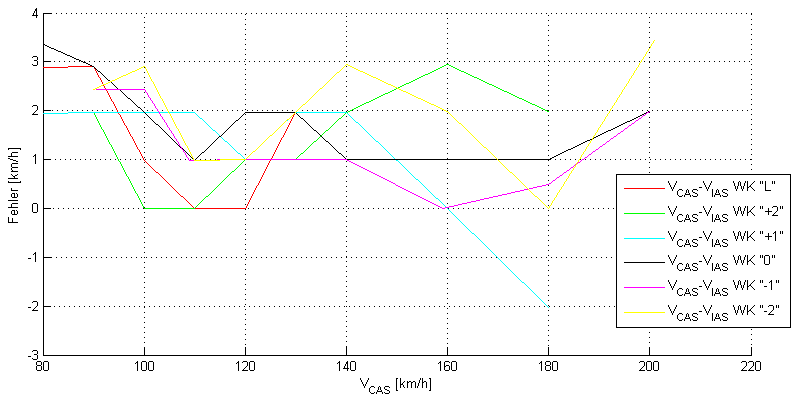
\includegraphics[width=.9\textwidth]{fahrtmesserkalibrierung.png}
\newline
Der Fehler der Fahrtmesseranlage beträgt nicht mehr als $8 \frac{km}{h}$ bzw. $5\%$ und erfüllt damit die Anforderungen der JAR 22 (siehe JAR 22.1323).

\section{Überziehgeschwindigkeiten}

Die folgenden Überziehgeschwindigkeiten wurden bei einem Abfluggewicht von $\unit[820]{kg}$ und vorderster Schwerpunktlage ermittelt:

\begin{tabular}{l l l}
WK $-2$ & & \\
& Geradeaus: & $\unit[78]{\frac{km}{h}}$\\
& $5^{\circ}$ schiebend: & $\unit[78]{\frac{km}{h}}$\\
& $45^{\circ}$-Kurve: & $\unit[95]{\frac{km}{h}}$\\
%& &  \\
\hline
& &  \\
WK $-1$ & & \\
& Geradeaus: & $\unit[79]{\frac{km}{h}}$\\
& $5^{\circ}$ schiebend: & $\unit[79]{\frac{km}{h}}$\\
& $45^{\circ}$-Kurve: & $\unit[88]{\frac{km}{h}}$\\
%& &  \\
\hline
& &  \\
WK $0$ & & \\
& Geradeaus: & $\unit[79]{\frac{km}{h}}$\\
& $5^{\circ}$ schiebend: & $\unit[79]{\frac{km}{h}}$\\
& $45^{\circ}$-Kurve: & $\unit[90]{\frac{km}{h}}$\\
%& &  \\
\hline
& &  \\
WK $+1$ & & \\
& Geradeaus: & $\unit[77]{\frac{km}{h}}$\\
& $5^{\circ}$ schiebend: & $\unit[77]{\frac{km}{h}}$\\
& $45^{\circ}$-Kurve: & $\unit[89]{\frac{km}{h}}$\\
%& &  \\
\hline
 & & \\
WK $+2$ & & \\
& Geradeaus: & $\unit[76]{\frac{km}{h}}$\\
& $5^{\circ}$ schiebend: & $\unit[76]{\frac{km}{h}}$\\
& $45^{\circ}$-Kurve: & $\unit[85]{\frac{km}{h}}$\\
%& &  \\
\hline
& &  \\
WK L& & \\
& Geradeaus: & $\unit[75]{\frac{km}{h}}$\\
& $5^{\circ}$ schiebend: & $\unit[75]{\frac{km}{h}}$\\
& $45^{\circ}$-Kurve: & $\unit[88]{\frac{km}{h}}$\\
& geradeaus, Bremsklappe + Fahrwerk aus: & $\unit[78]{\frac{km}{h}}$ \\
\end{tabular}
\section{Fahrtmessermarkierungen}
Die folgende Tabelle nennt die Fahrtmessermarkierungen und die Bedeutung der Farben:\\

\begin{tabular}{|m{1,8cm}|m{1,5cm}|m{6cm}|}
\hline
Markierung & IAS [$\unit{\frac{km}{h}}$] & Bedeutung \\
\hline
Weißer Bogen & $80-180$ & Betriebsbereich für positive Klappenausschläge (Untere Grenze ist die Geschwindigkeit $1,1 \cdot V_{S0}$ bei Höchstmasse in Landekonfiguration. Obere Grenze ist die zulässige Höchstgeschwindigkeit mit positivem Klappenausschlag.)\\
\hline
\begin{color}{forestgreen} Grüner Bogen \end{color} & \begin{color}{forestgreen} $80-180$ \end{color} & \begin{color}{forestgreen} Normaler Betriebsbereich (Untere Grenze ist die Geschwindigkeit $1,1 \cdot V_{S1}$ bei Höchstmasse und vorderster Schwerpunktlage und Flügelklappen in der Neutralstellung; obere Grenze ist die zulässige Höchstgeschwindigkeit in starker Turbulenz) \end{color} \\ 
\hline
\begin{color}{myyellow} Gelber Bogen \end{color} & \begin{color}{myyellow} $180-220$ \end{color} & \begin{color}{myyellow} In diesem Bereich darf bei starker Turbulenz nicht geflogen werden und Manöver dürfen nur mit Vorsicht durchgeführt werden. \end{color}\\
\hline
\begin{color}{red} Roter Strich \end{color} & \begin{color}{red} $220$ \end{color} & \begin{color}{red} Zulässige Höchstgeschwindigkeit für alle Betriebsarten \end{color}\\
\hline
\begin{color}{myyellow} Gelbes Dreieck \end{color} & \begin{color}{myyellow} $95$ \end{color} & \begin{color}{myyellow} Anfluggeschwindigkeit bei Höchstmasse \end{color}\\
\hline
\end{tabular}
\newline

\vspace{0.2cm}
Die B13 hat keine speziellen Fahrmessermarkierungen für den Motorbetrieb.
\newpage
\section{Triebwerk}
\begin{color}{red}
\large{\underline{Warnung}}\\
Die B13 ist nicht für den Eigenstart zugelassen.
\end{color}\\

\subsection{Motor}
\begin{tabular}{p{0.3\textwidth}p{0.6\textwidth}ll}
Motor Hersteller: & Emrax d.o.o.\\
Motor Modell: & Emrax 208 LowVoltage AirCooled\\
\end{tabular}\\

\vspace{0.2cm}
\begin{tabular}{p{0.6\textwidth}p{0.3\textwidth}ll}
Maximale Dauerleistung: & $\unit[22]{kW}$\\
Maximale Leistung für 2 Minuten: & $\unit[30]{kW}$\\
Maximale Drehzahl: & $\unit[5000]{1/min}$
\end{tabular}

\subsection{Propeller}
\begin{tabular}{p{0.3\textwidth}p{0.5\textwidth}ll}
Hersteller: & Akaflieg Berlin e.V. \\
Modell: & B13e Faltpropeller V01 \\
\end{tabular}\\

\vspace{0.2cm}
\begin{tabular}{p{0.6\textwidth}p{0.3\textwidth}ll}
Maximale Dauerdrehzahl: & $\unit[3000]{u/min}$ \\
Kurzzeitige Überdrehzahl: & $\unit[3200]{u/min}$ \\
\end{tabular}

\subsection{Akkupacks}
\begin{tabular}{p{0.4\textwidth}p{0.5\textwidth}ll}
Hersteller: & LZ-Design d.o.o \\
Bezeichnung:& FES GEN2 75Ah \\
\end{tabular}\\

\vspace{0.2cm}
Das Antriebsystem benötigt zwei in Reihe geschaltete Akkupacks. Jedes Akkupack besitzt 14 LiPo Zellen, also insgesamt 28 Zellen.\\

\begin{tabular}{p{0.83\textwidth}p{0.15\textwidth}ll}
Max. zulässige Gesamtspannung beider Akkupacks: & $\unit[118]{V}$ \\
Min. zulässige Gesamtspannung beider Akkupacks: & $\unit[90]{V}$ \\
Nennkapazitat pro Zelle: & $\unit[75]{Ah}$ \\
Energiespeicherkapazitat: & $\unit[7,8]{kWh}$ \\
Maximale Spannung pro Zelle: & $\unit[4,16]{V}$ \\
Nennspannung: & $\unit[3,7]{V}$ \\
Minimale Spannung pro Zelle: & $\unit[3,2]{V}$ \\
\end{tabular}\\

\vspace{0.5cm}
Weitere Informationen über die verwendeten Akkupacks finden Sie im \textbf{FES AKKUPACKHANDBUCH der Firma LZ-Design.}

\section{Markierungen des Triebwerksinstruments}
Das FES Triebwerk besitzt ein FCU Instrument mit einem hochauflösenden
sonnenlichtgeeignetem Farbdisplay. Weitere Informationen über die FCU und Ihre
Bedienung finden Sie im \textbf{FES FCU INSTRUMENTENHANDBUCH!}

\section{Masse (Gewicht)}
\begin{tabular}{l l}
Leermasse & s. Wägebericht\\
Höchstzulässige Abflugmasse & $\unit[820]{kg}$\\
Höchstzulässige Masse nichttragender Teile & $\unit[506]{kg}$ \\
Höchstmasse im Gepäckraum & $\unit[10]{kg}$ \\
\end{tabular}\\

\vspace{0.5cm}
Die Masse der Batterie Packs beträgt insgesamt ca. $\unit[50]{kg}$, der Antriebsstrang mit Motor und Propeller wiegt $\unit[19]{kg}$, der Regler wiegt ca. $\unit[5]{kg}$.\\

\begin{color}{red}
\large{\underline{Warnung}}\\
Die Mindestzuladung ohne Motor und ohne Batterien beträgt ca. $\unit[150]{kg}$!
\end{color}\\


\section{Schwerpunkt}
\begin{tabular}{l l}
Flugzeuglage & Keil $1000:28$ auf der Rumpfoberseite\\
Bezugsebene (BE) & Flügelvorderkante an der Wurzelrippe \\
Größte Vorlage & $\unit[245,3]{mm}$ hinter BE\\
Größte Rücklage & $\unit[428,6]{mm}$ hinter BE\\
\end{tabular}\\

\vspace{0.5cm}
\textbf{Hebelarme}\\
\begin{tabular}{m{6,5cm} m{3cm}}
Piloten & $x_P=\unit[-445]{mm}$\\
Gepäckfach & $x_G=\unit[200]{mm}$\\
\end{tabular}\\

Die Bezugsebene ist die Vorderkante der Wurzelrippe.\\

Die Antriebskomponenten der B13 wurden so positioniert, dass ein großer Zuladungsbereich möglich ist. \\


\begin{color}{red}
\large{\underline{Warnung}}\\
Ein Flug mit ausgebautem Motor ist nur in Verbindung einer neuen Wägung zulässig. Ein Ausbau des Antriebsstrangs erhöht in deutlichem Maße die Mindestzuladung.
\end{color}\\


\begin{color}{red}
\large{\underline{Warnung}}\\
Ein Flug mit ausgebautem Akkupack ist nur in Verbindung einer neuen Wägung zulässig. Ein Ausbau der Akkupacks erhöht in deutlichem Maße die Mindestzuladung.
\end{color}\\

\subsection{Wägebericht}

\begin{tiny}
\begin{tabular}{|m{1,8cm}|m{1,8cm}|m{2cm}|m{1,5cm}|m{1,5cm}|}
\hline
Datum & Leermasse [$\unit{kg}$] & Leermassen- schwerpunkt [$\unit{mm}$]  & Maximale Zuladung [$\unit{kg}$] & Unterschrift\\

\hline
& & & &\\
14.03.12 & 579 & 552,9 & 221 & Hofmann\\
& & & &\\
\hline
& & & &\\
23.02.19 & 655 & 514 & 165 & Döring\\
& & & &\\
\hline
& & & &\\
& & & &\\
& & & &\\
\hline
& & & &\\
& & & &\\
& & & &\\
\hline
& & & &\\
& & & &\\
& & & &\\
\hline

\end{tabular}
\end{tiny}

%\newline
%Weitere Hinweise zur Schwerpunktlage und dem Beladeplan sind dem Kapitel 6 "`Masse und Schwerpunktlage"' zu entnehmen.

\section{Zugelassene Manöver}
Der Motorsegler B13 ist für den normalen Segelflug (Lufttüchtig"-keits"-gruppe "`Utility"') zugelassen.\\
\newline
\begin{color}{red}
\textbf{Kunstflug ist nicht zulässig}
\end{color}

\section{Manöverlastvielfache}

Folgende Lastvielfache dürfen beim Abfangen nicht überschritten werden.\\
\newline
\begin{tabular}{|l|c|c|}
\hline
& positiv & negativ \\
\hline
Bei Manövergeschwindigkeit $V_A=\unit[160]{\frac{km}{h}}$ & $+5,3$ & $-2,65$\\
\hline
Bei Höchstgeschwindigkeit $V_{NE}=\unit[220]{\frac{km}{h}}$ & $+4,0$ & $-1,5$ \\
\hline
Bei ausgefahrenen Bremsklappen und $V_{NE}$ & $+3,5$ & $0$\\
\hline
\end{tabular}

\section{Flugbesatzung}
Die B13 kann einsitzig oder doppelsitzig geflogen werden. Der verantwortliche Luftfahrzeugführer kann auf der linken oder rechten Seite sitzen. Es wird empfohlen, die Platzrunde und insbesondere bodennahe Kurven (z.B. bei Seilriss) in Richtung des fliegenden Luftfahrzeugführes auszuführen, da ansonsten mit Sichtbeeinträchtigungen gerechnet werden muss.

\section{Betriebsarten}
Mit der B13 dürfen Flüge nach Sichtflugregeln (VFR) bei Tag durchgeführt werden.\\
\newline
\begin{color}{red} \large{\underline{Warnung}}\\
Kunstflug und Wolkenflug sind nicht zulässig
\end{color}\\

\begin{color}{red}
\large{\underline{Warnung}}\\
Flüge bei starkem Regen mit laufendem Motor sind verboten! Es
muss sichergestellt werden, dass die Bestandteile des Elektroantriebes nicht nass werden.
\end{color}\\

\begin{color}{red}
\large{\underline{Warnung}}\\
Eigenstarts mit der B13 sind nicht zulässig.
\end{color}
\newpage
\section{Mindestausrüstung}
Zur Mindestausrüstung für den Normalbetrieb gehören:\\
\begin{itemize}
\item Fahrtmesser (bis $\unit[300]{\frac{km}{h}}$ mit Farbmarkierungen nach Abschnitt 2.3)
\item Höhenmesser
\item Variometer
\item Magnetkompass
\item 2 Anschnallgurte (vierteilig, symmetrisch)
\item Flug- und Betriebshandbuch
\item Daten- und Hinweisschilder
\item 2 automatische oder manuelle Fallschirme
\end{itemize}

\section{Flugzeugschlepp und Windenschlepp}

\textbf{Flugzeugschlepp}\\
Die maximal zulässige Schleppgeschwindigkeit beträgt $V_T=\unit[160]{\frac{km}{h}}$.\\
Es wurden Seillängen zwischen $\unit[30]{m}$ und $\unit[60]{m}$ erprobt.\\
Die Sollbruchstellen des Schleppseils sollten eine Bruchlast von $\unit[1000]{daN}$ (schwarz) erreichen.\\
Für den Flugzeugschlepp wird die Schwerpunktkupplung an der Rumpfunterseite verwendet.\\

\textbf{Windenschlepp}\\
Die maximal zulässige Schleppgeschwindigkeit beträgt $V_W=\unit[120]{\frac{km}{h}}$, $\unit[100]{\frac{km}{h}}$ sollte nicht unterschritten werden.\\
Die Sollbruchstellen des Windenseils sollten eine Bruchlast von $\unit[1000]{daN}$ (schwarz) haben.\\
Für den Windenstart wird die Schwerpunktkupplung an der Rumpfunterseite verwendet.
\newpage

\section{Hinweisschilder für Betriebsgrenzen}

\begin{figure}[h]
\begin{center}
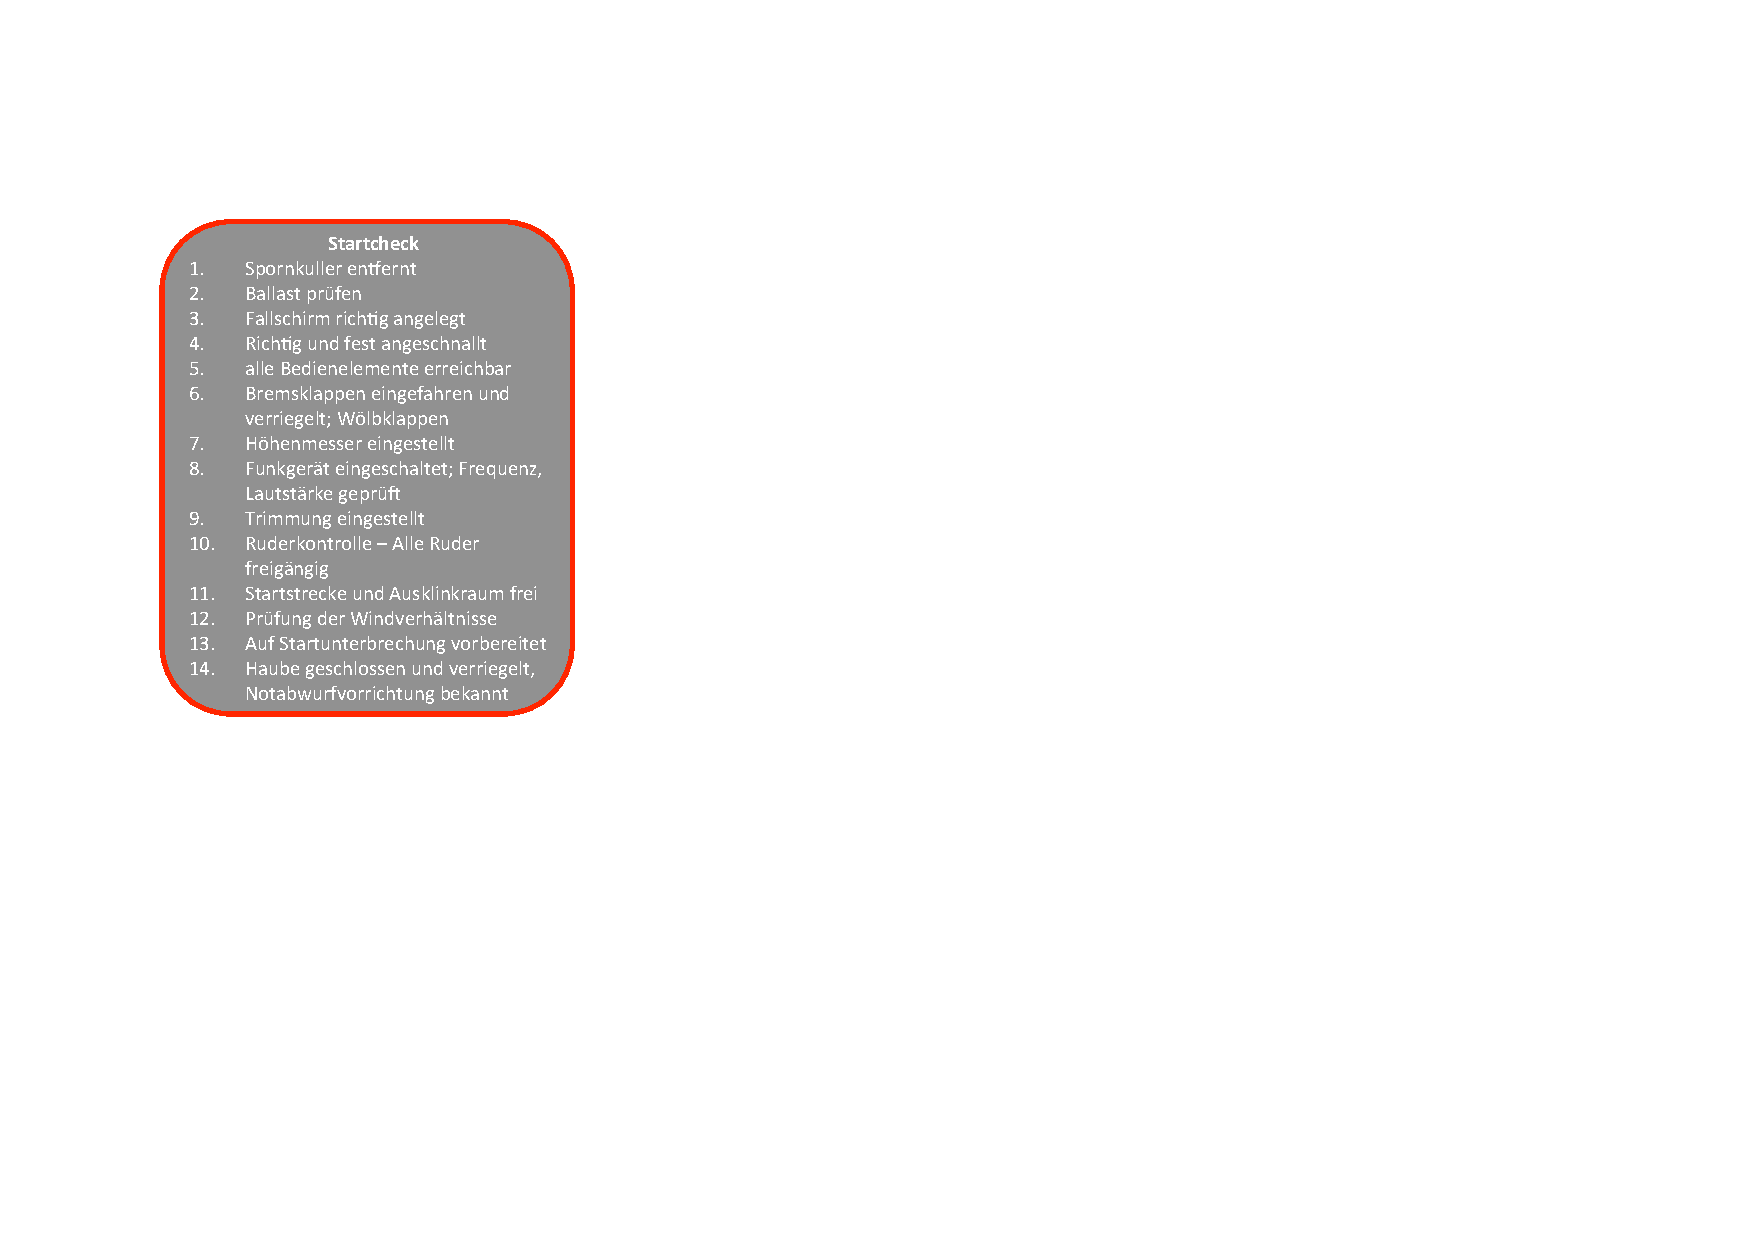
\includegraphics[width=.45\textwidth]{bilder/startcheck.pdf}
\caption*{Startcheck}
\end{center}
\end{figure}

\begin{figure}[h]
\begin{center}

\includegraphics[width=.9\textwidth]{bilder/vvz.pdf}
\caption*{Permit To Fly}
\end{center}
\end{figure}

\begin{figure}[H]
\begin{center}
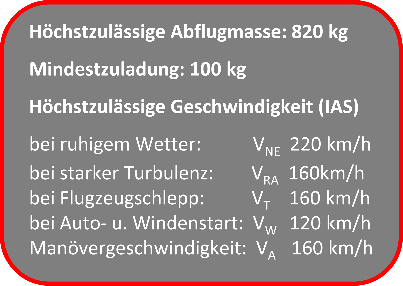
\includegraphics[width=.45\textwidth]{bilder/datenschild.pdf}
\caption*{Datenschild}
\end{center}
\end{figure}

\begin{figure}[H]
\begin{center}
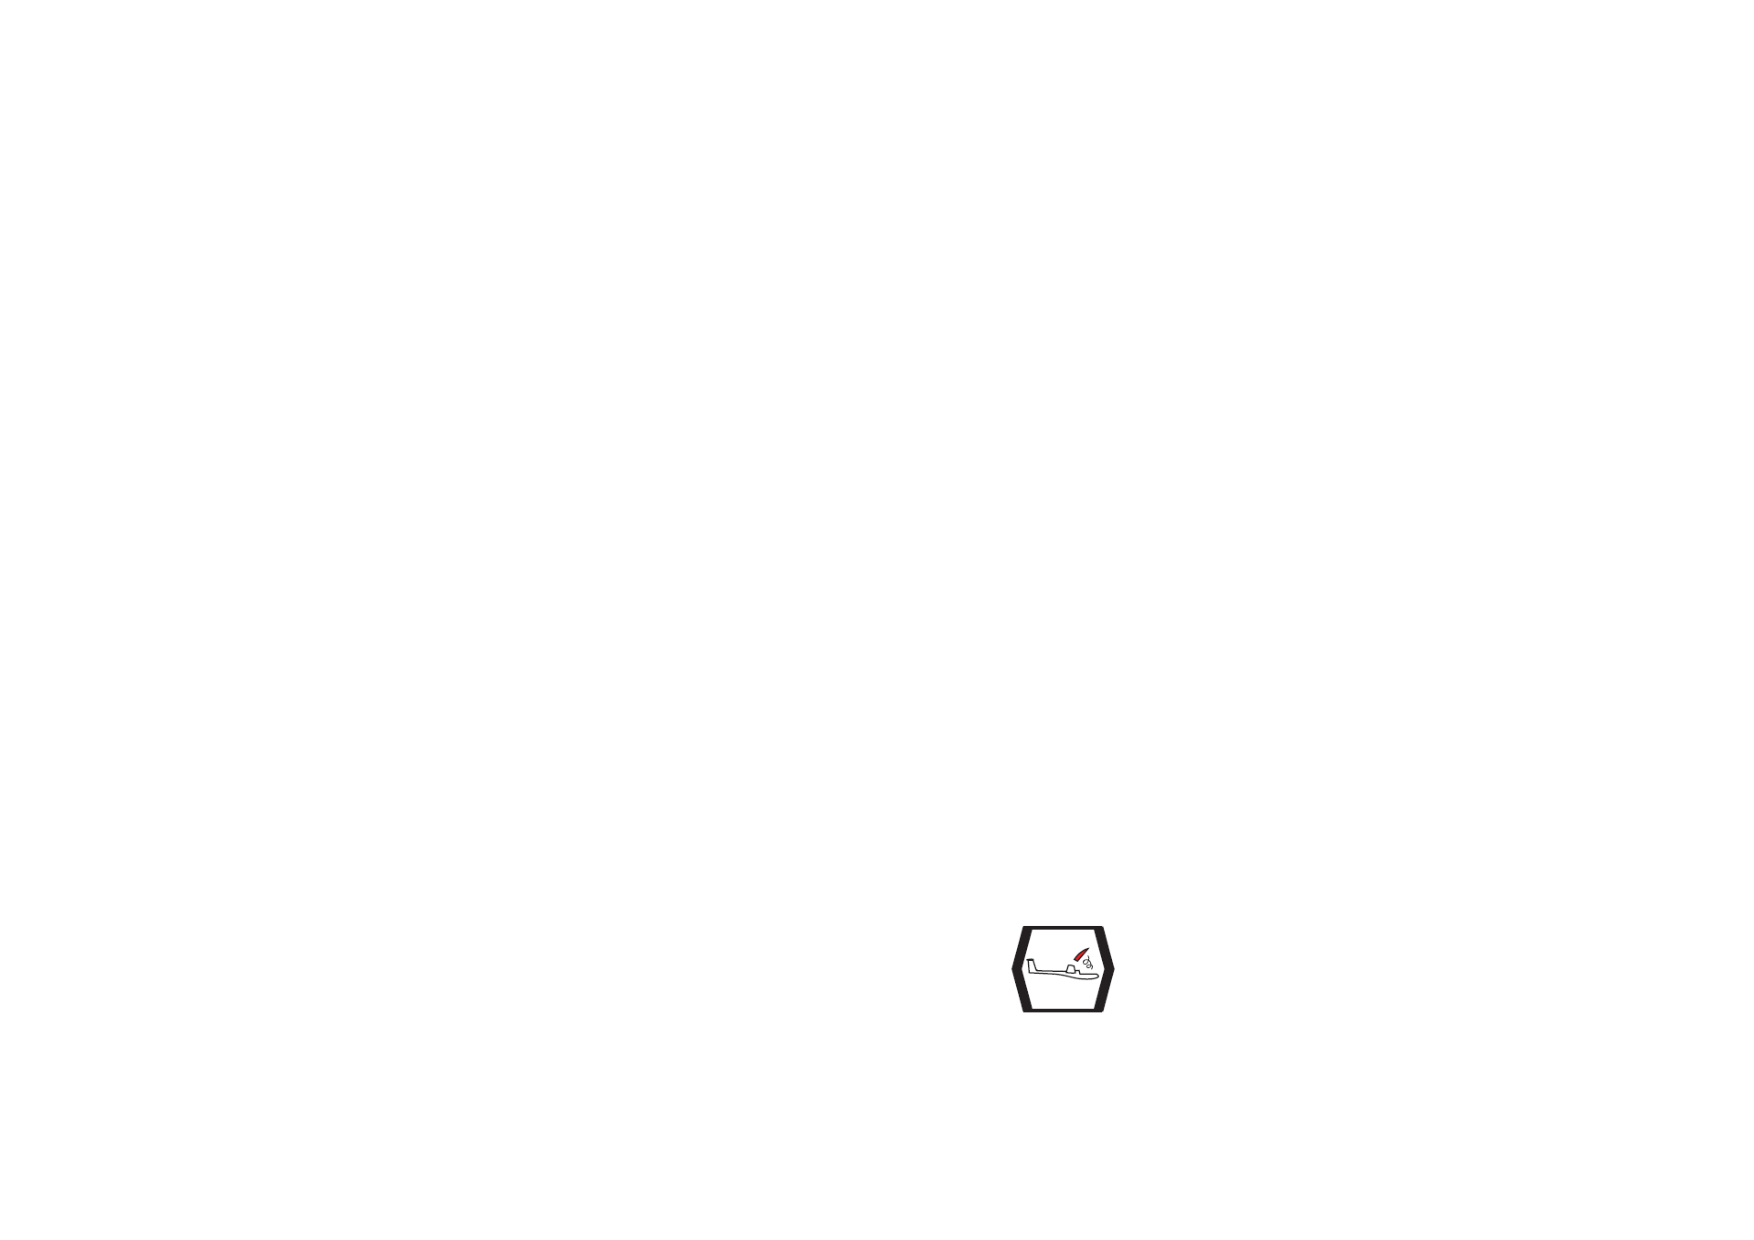
\includegraphics[width=.15\textwidth]{bilder/notabwurf.pdf}\\
\caption*{Haubennotabwurf am Instrumentenbrett}
\end{center}
\end{figure}

\begin{figure}[H]
\begin{center}
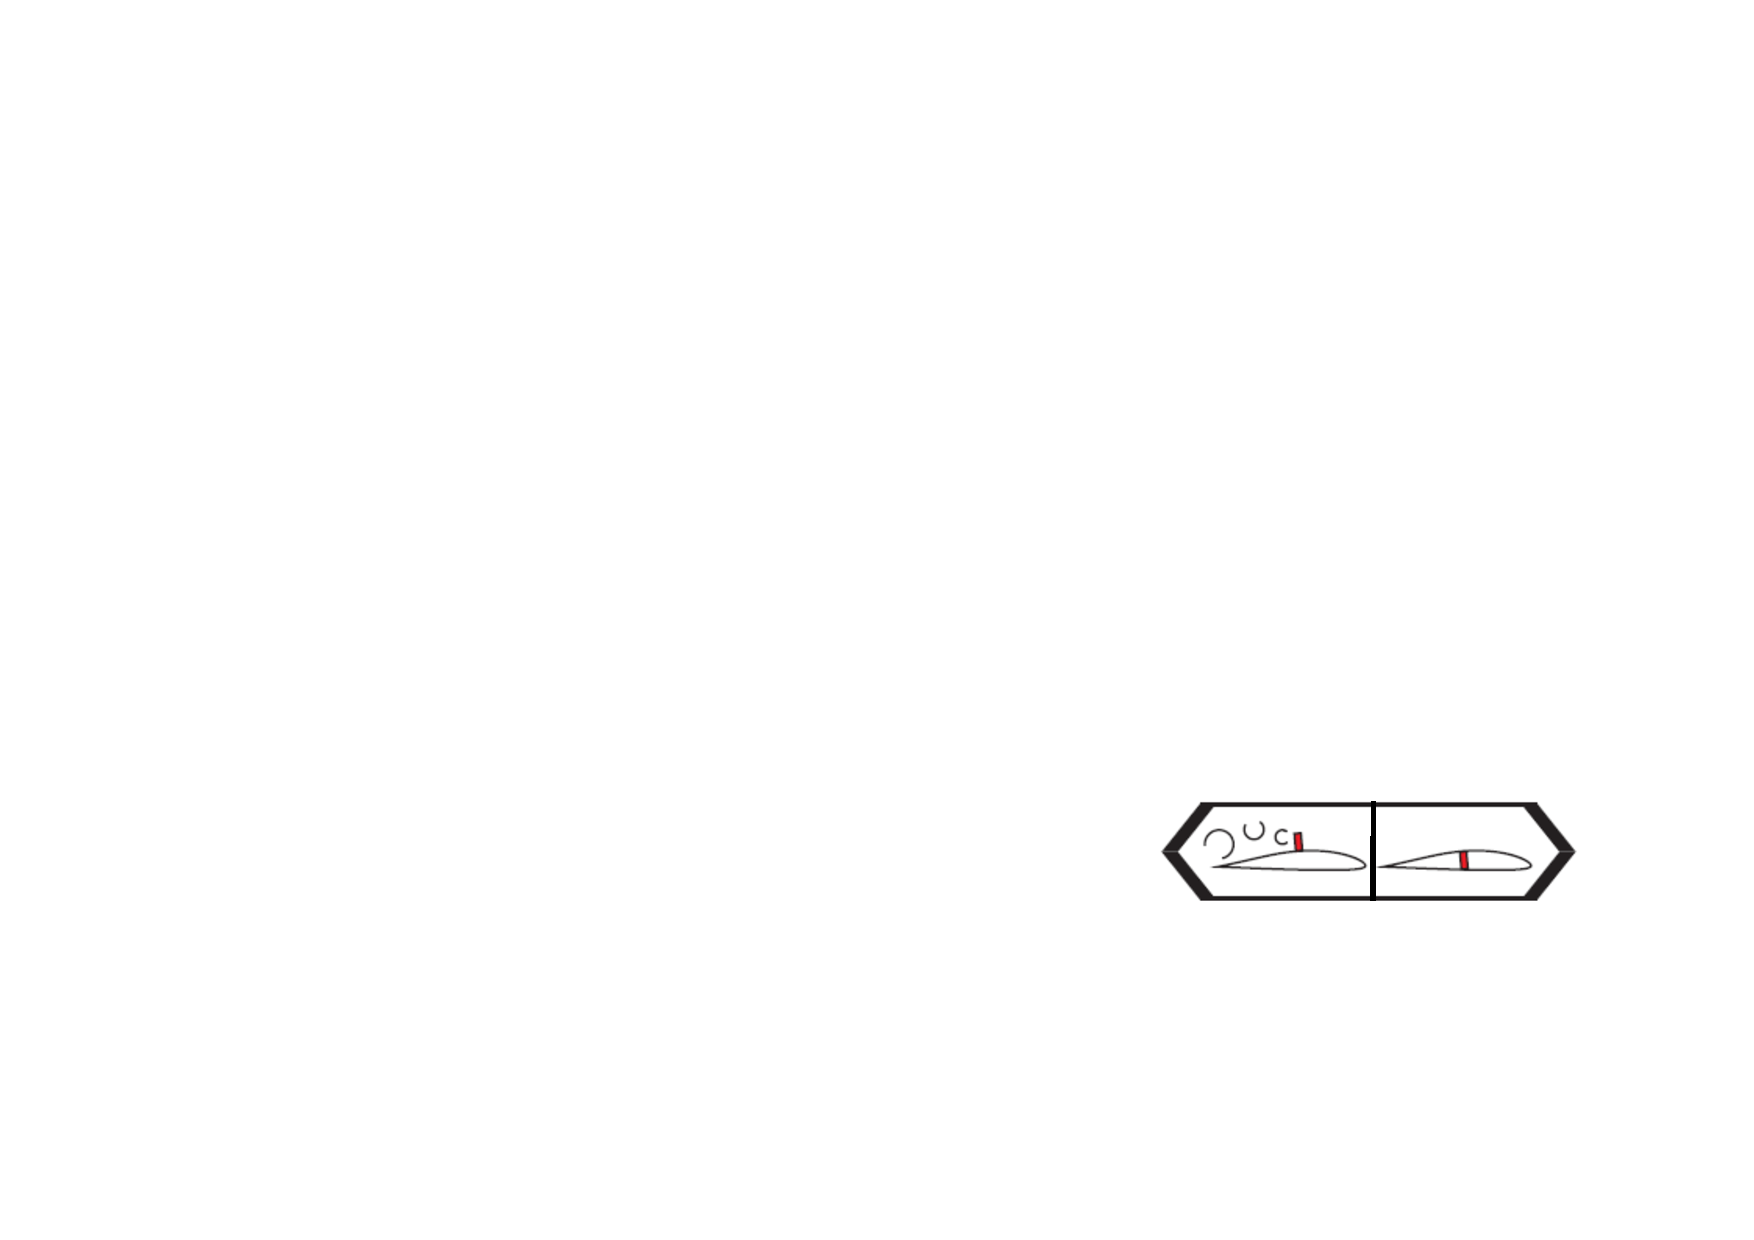
\includegraphics[width=.45\textwidth]{bilder/bk.pdf}
\caption*{Bremsklappen, blauer Griff jeweils links}
\end{center}
\end{figure}


\begin{figure}[H]
\begin{center}
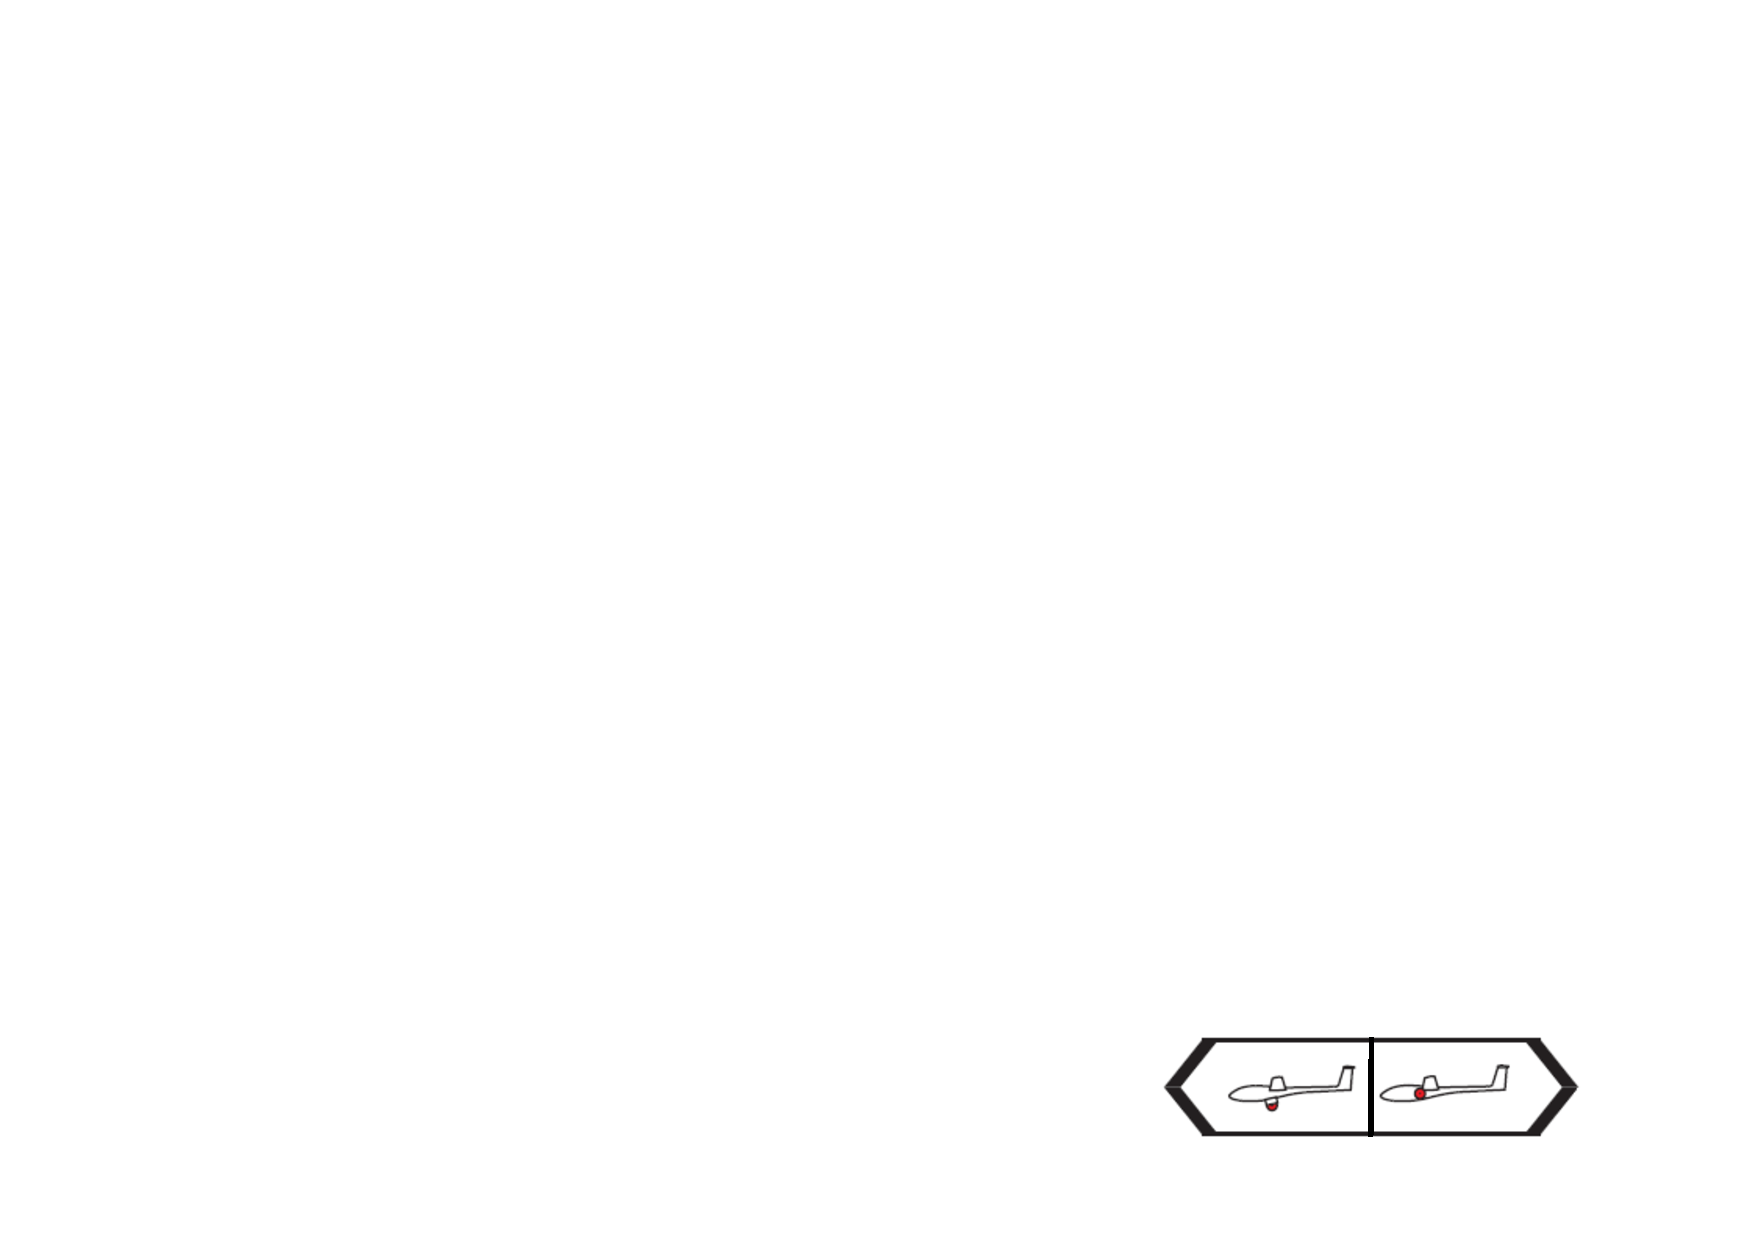
\includegraphics[width=.45\textwidth]{bilder/fahrwerk.pdf}
\caption*{Fahrwerk, silberner Hebel in der Mitte}
\end{center}
\end{figure}

\begin{figure}[H]
\begin{center}
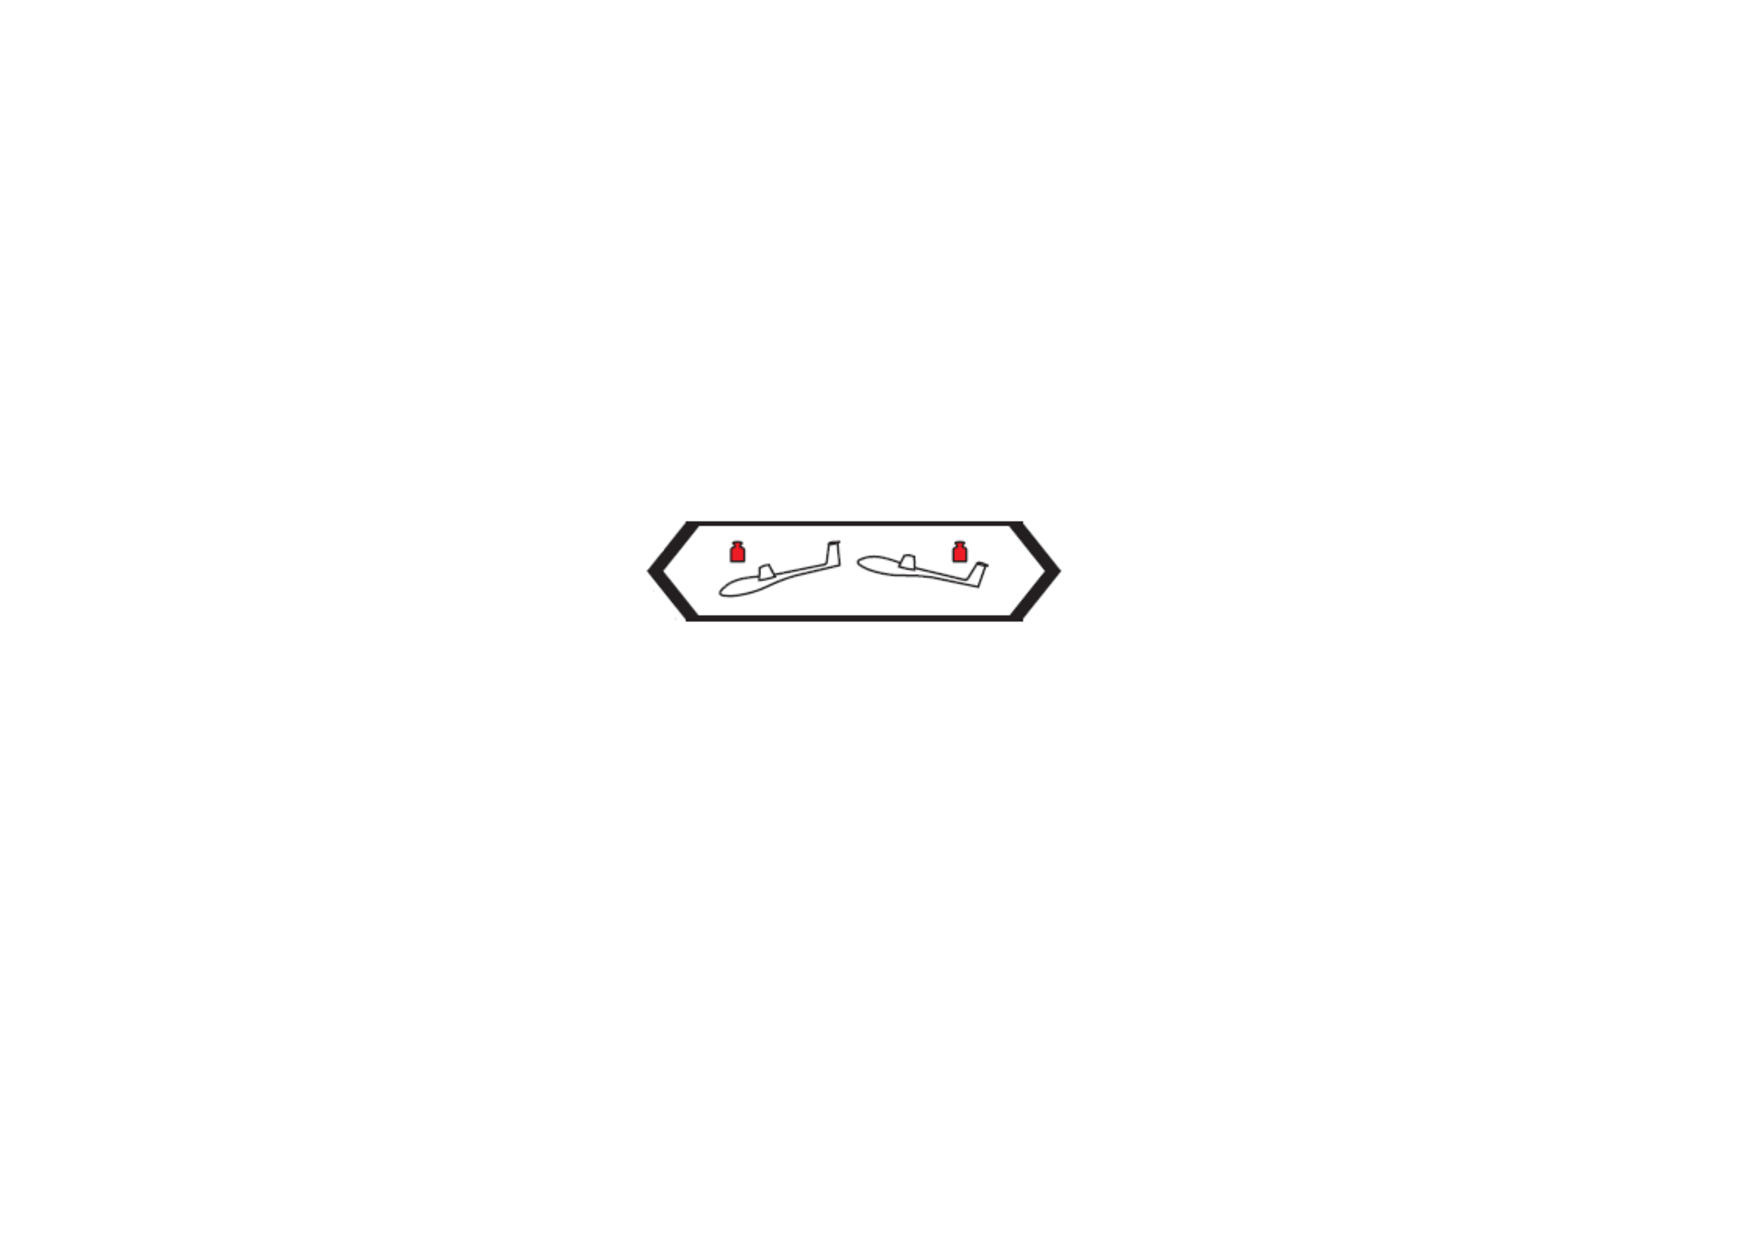
\includegraphics[width=.45\textwidth]{bilder/trimmung.pdf}
\caption*{Trimmung, grüner Hebel in der Mitte}
\end{center}
\end{figure}

\begin{figure}[H]
\begin{center}
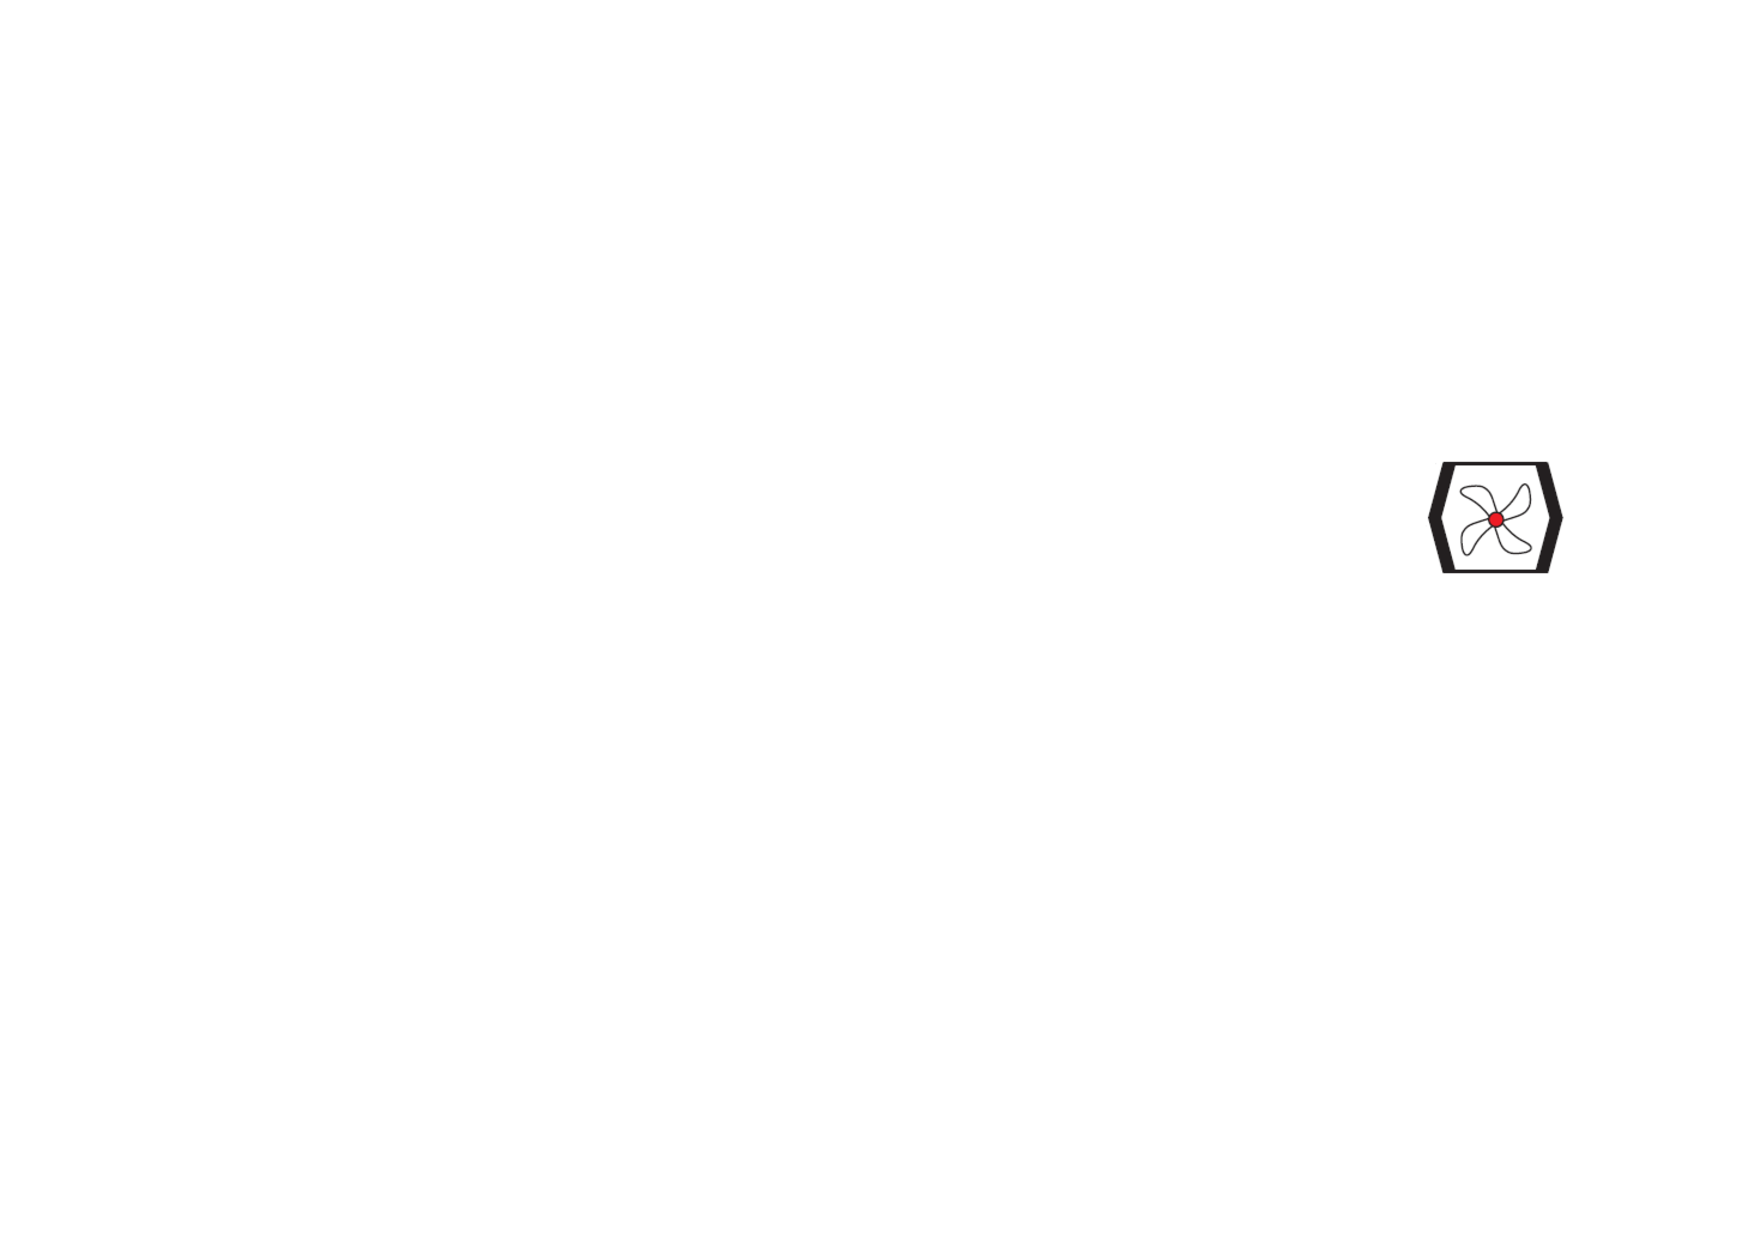
\includegraphics[width=.15\textwidth]{bilder/lueftung.pdf}
\caption*{Lüftungsbetätigung, Knopf links und rechts an Cockpitwand}
\end{center}
\end{figure}

\begin{figure}[H]
\begin{center}
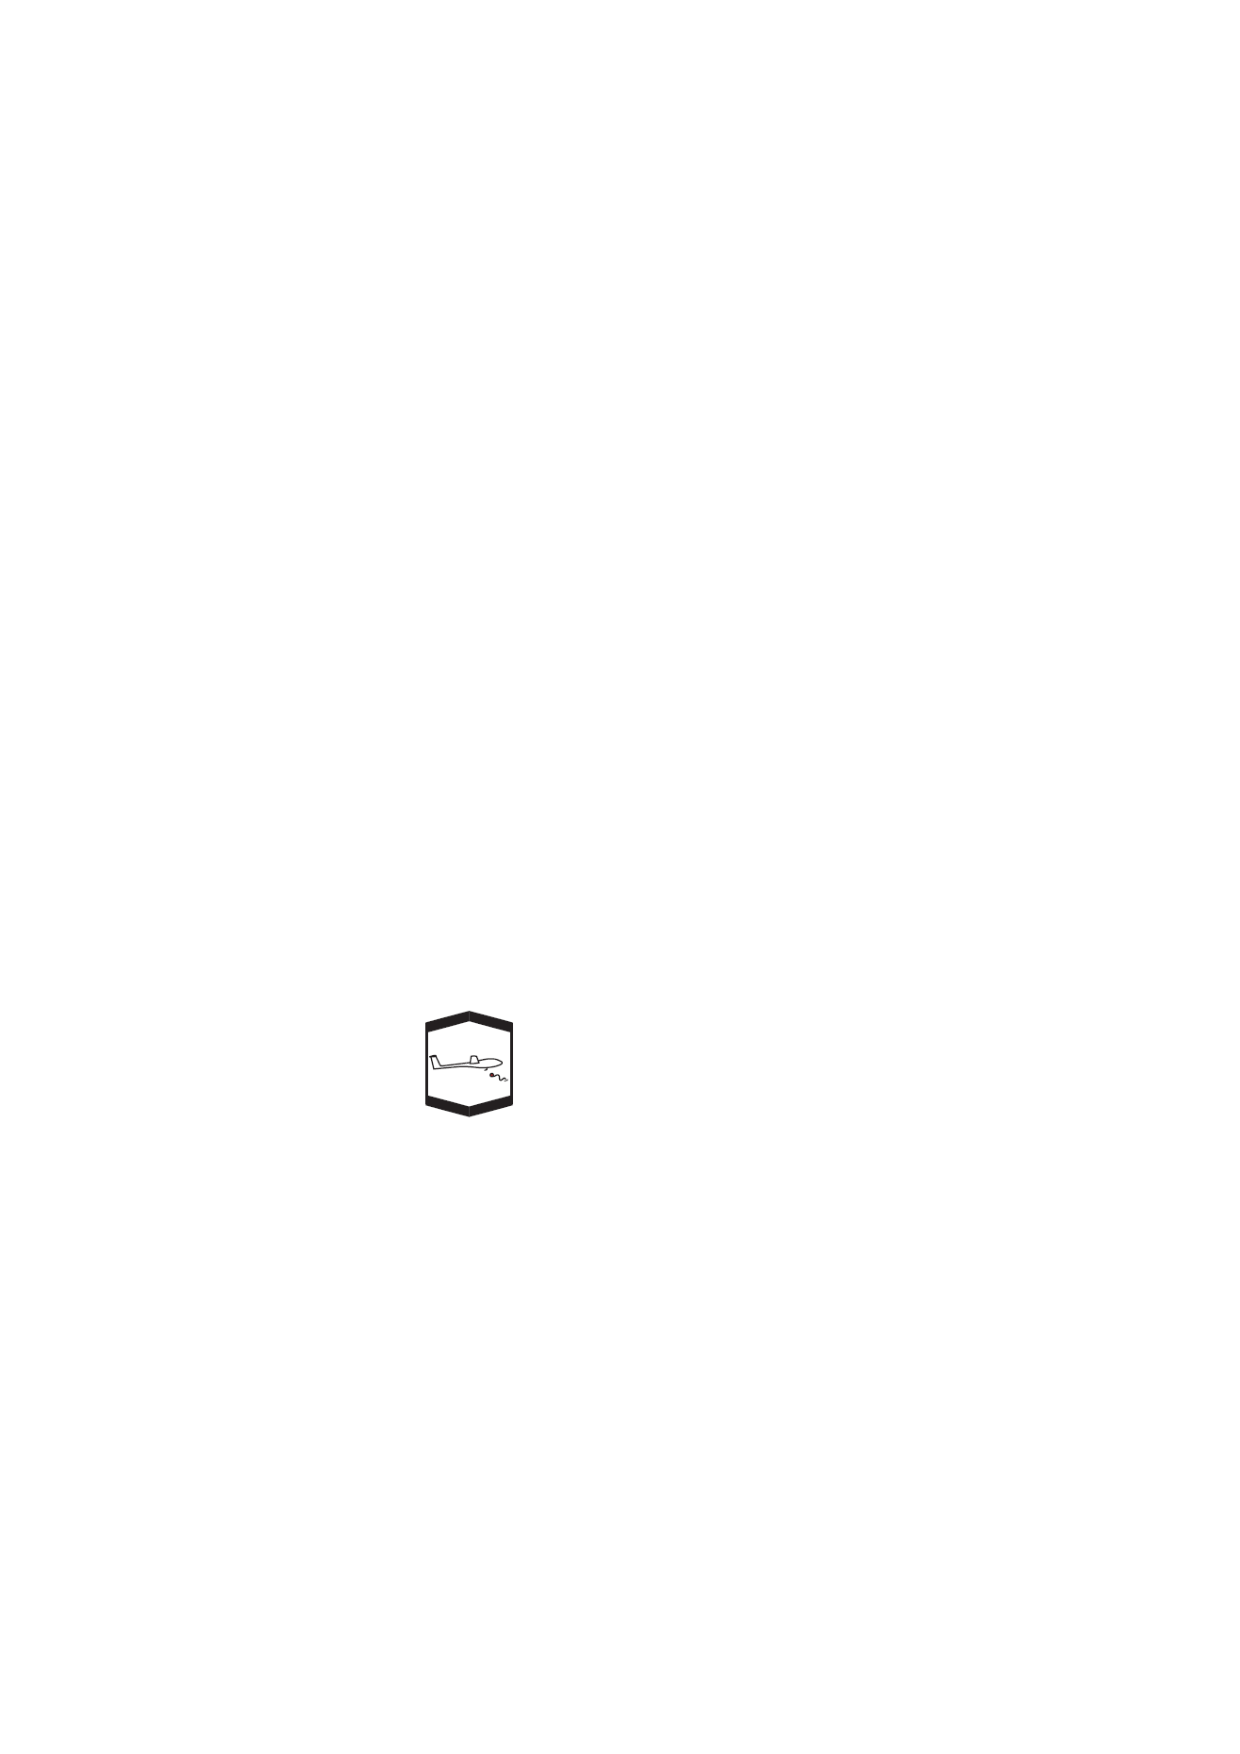
\includegraphics[width=.15\textwidth]{bilder/kupplung.pdf}
\caption*{Schleppkupplung, gelber Griff jeweils links neben Steuerknüppel}
\end{center}
\end{figure}

\begin{figure}[H]
\begin{center}
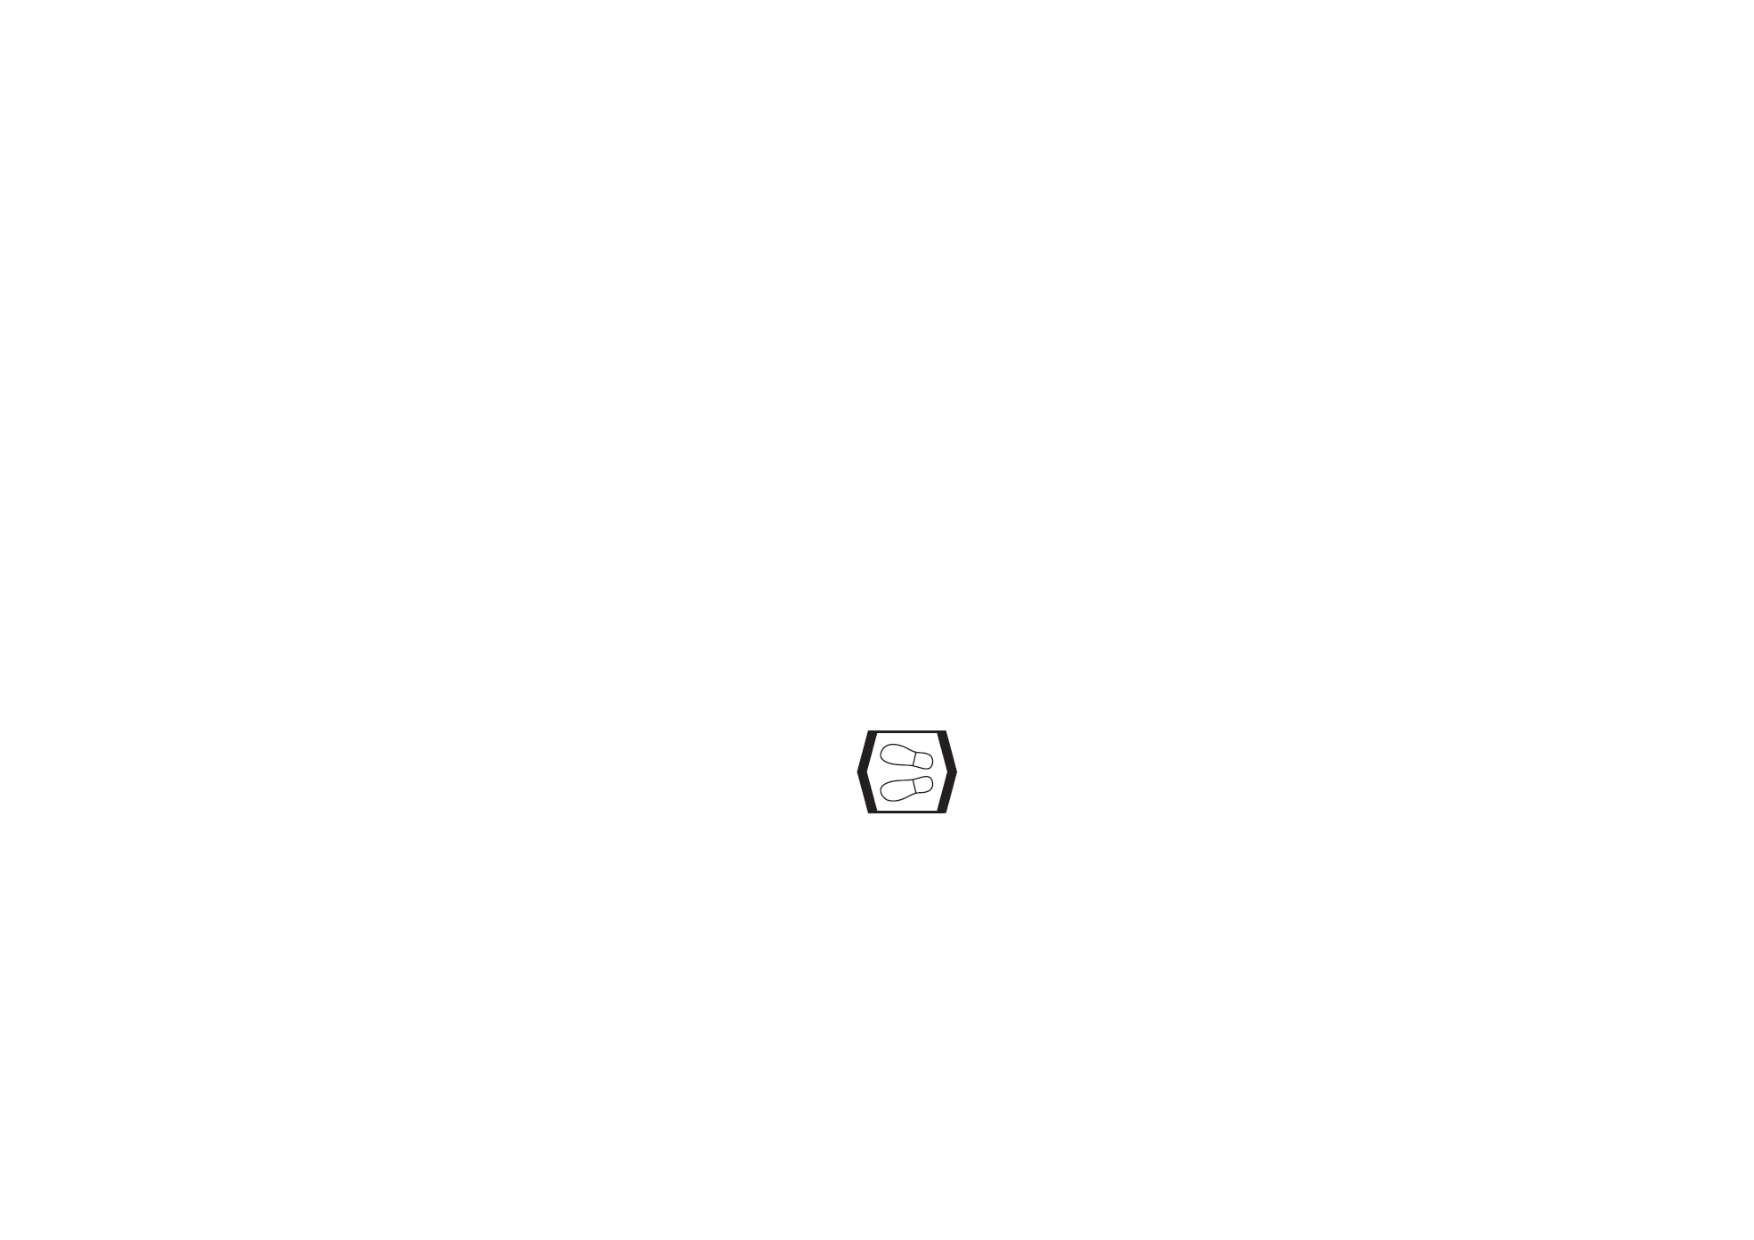
\includegraphics[width=.15\textwidth]{bilder/pedale.pdf}
\caption*{Pedalverstellung, weißer Griff rechts neben Steuerknüppel}
\end{center}
\end{figure}

\begin{figure}[H]
\begin{center}
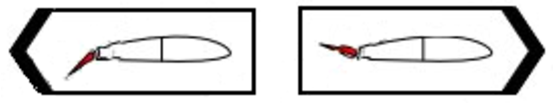
\includegraphics[width=.45\textwidth]{bilder/wk.pdf}
\caption*{Wölbklappenhebel, schwarzer Griff, jeweils links}
\end{center}
\end{figure}

Zusätzliche Hinweisschilder müssen für mit einem FES System ausgestattete
Segelflugzeuge hinzugefügt werden:\\

\begin{center}
\begin{tabular}[H]{|l|l|l|}
\hline
\multicolumn{2}{|l|}{\textbf{Geschwindigkeit IAS:}} & Km/h \\
\hline
Triebwerksbetrieb & $V_\text{PO}$ & 80-160 \\
\hline
Max. Motor Start/Stopp & $V_\text{POmax}$ & 135 \\
\hline
\end{tabular}
\end{center}


